% Chapter Template

\chapter{Método} % Main chapter title

\label{Cap_Exp} % Change X to a consecutive number; for referencing this chapter elsewhere, use \ref{ChapterX}

%----------------------------------------------------------------------------------------
%	SECTION 1
%----------------------------------------------------------------------------------------
\section{Planteamiento general: Explorando la generalizabilidad del Efecto Espejo}

%Se propone buscar evidencia del Efecto Espejo en una tarea fuera de Memoria de reconocimiento.
Al tratarse de un fenómeno exclusivamente reportado, estudiado e interpretado dentro de la literatura en Memoria de Reconocimiento, existe una tendencia a explicar el Efecto Espejo -las diferencias en la ejecución de los participantes entre las clases de estímulos contenidos en el experimento- apelando a posibles discrepancias en el procesamiento superior de los mismos durante la fase de estudio (por ejemplo, la atención, la recolección de rasgos para su futuro reconocimiento, etc.). El interés principal de la investigación aquí reportada fue buscar evidencia de los patrones de respuesta reportados en estudios de Memoria de Reconocimiento en una tarea de detección ajena a dicha área.\\

%Encontrar evidencia del Efecto Espejo en otra área, podría sugerir que el Efecto Espejo es resultado del uso de SDT para comparar dos condiciones de discriminabilidad y no necesariamente de un fenómeno de Memoria per see.
Buscar evidencia del Efecto Espejo fuera del área de Memoria de Reconocimiento permite evaluar la posibilidad de que los patrones de respuesta reportados como parte del mismo sean producto de la aplicación de la TDS como marco para el análisis y comparación de la ejecución de los participantes entre clases de estímulos que difieren en su discriminabilidad y no necesariamente de una discrepancia en su procesamiento durante la fase de estudio.\\

%Se propone una tarea perceptual ya que carece de una fase de preparacion. Se trabaja con ilusiones opticas, dado que la literatura en ellas permite anticiparnos a la d' y proponer dos niveles de dificultad.
Se decidió trabajar con una tarea de detección perceptual por dos grandes razones. La primera razón es que una tarea de este tipo implica un procedimiento más sencillo: los participantes deciden si la señal está o no presente en los estímulos mostrados sin haber interactuado con estos en una etapa previa. La señal a detectar se percibe en el estímulo, no se reconoce de la experiencia previa con el mismo. La segunda razón es que existe un cuerpo de literatura lo suficientemente amplio como para permitir la construcción de dos niveles de dificultad dentro de la tarea, específicamente, se revisó y trabajó con la literatura que aborda el fenómeno de las ilusiones ópticas.\\

\subsection{Objetivo}

%Buscar evidencia del efecto espejo en una tarea de detección perceptual.
Determinar si los patrones de respuesta identificados como parte del Efecto Espejo en Memoria de Reconocimiento aparecen también al coparar el desempeño de los participantes entre distintos niveles de discriminabilidad en una tarea de detección perceptual.\\

\section{Construcción de los Experimentos}

%5.	Jaeger, T., & Pollack, R. (1977). Effect of contrast level and temporal order on the Ebbinghaus circles illusion. Perception & Psychophysics. Vol 21 (1), 83-97.
%9.	Pressey, A. (1977). Measuring the Titchener circles and Delboeuf illusions with the method of adjustment. Bulletin of Psychonomic Society. Vol 10 (2), 118-120.
%Coren, S., & Girgus, J. (1978). Seeing is deceiving: The psychology of visual illusions. Hillsdale, NJ: Erlbaum.
%Titchener E B, 1901 Experimental Psychology: A Manual of Laboratory Practice volume I (London: MacMillan) (1901, page 169, figure 3)
%Robinson J O, 1972 The Psychology of Visual Illusion (London: Hutchinson Education)
%Rabin, J., & Adams, A. J. (1993). Size induction transcends the cardinal directions of color space. Perception, 22, 841–845.

%La tarea de detección consiste en identificar los ensayos donde el tamaño de dos círculos en pantalla es igual. Esta tarea tiene dos variaciones: En el Experimento 1, uno de los círculos a comparar es el círculo central de una ilusión de Ebbinghaus; En el Experimento 2, los dos círculos lo son. 
Se diseñó una tarea perceptual donde los participantes tenían que comparar el tamaño de dos círculos mostrados en pantalla y emitir una respuesta que señalara si los círculos tenían el mismo diámetro (señal) o no (ruido). Esta tarea se presentó en dos variaciones: En un primer caso, sólo uno de los círculos a comparar constituía el círculo central de una figura de Ebbinghaus (Experimento 1); En el segundo, ambos círculos aparecían como el componente central de una figura de Ebbinghaus distinta (Experimento 2).\\ 

%Descripcion de la Ilusión de Ebbinghausyhhhhhhhhhhvcf , la composición de la figura y cómo se explica.
La figura de Ebbinghaus -también conocida como Círculos de Titchner- está intrínsecamente relacionada con una ilusión óptica donde la percepción del tamaño de un elemento central es alterada por el contraste que tiene con elementos circundantes (la ilusión de Ebbinghaus). En la Figura~\ref{fig:Ebbinghaus} se presenta un par de ejemplos prototípicos de figuras con la ilusión de Ebbinghaus que demuestran las dos direcciones en que esta se puede presentar: la subestimación del tamaño de un estímulo (el círculo central) al estar rodeado por éstímulos más grandes (efecto de subestimación; figura izquierda), y la sobrestimación del tamaño de un estímulo rodeado por elementos de menor tamaño (efecto de sobrestimación; figura derecha); el diámetro de los círculos centrales en ambas figuras es el mismo. Esta ilusión perceptual suele explicarse como el reflejo de una tendencia en nuestro sistema a computar el tamaño de los objetos en función a su contraste con elementos similares en su entorno \parencite{Coren1971, Coren1974, Fockert2007}.\\

\begin{figure}[th]
\centering

\includegraphics[width=0.55\textwidth]{Figures/Ebbinghaus} 
\decoRule
\caption[Ilusión de Ebbinghaus: Ejemplos]{Ejemplos prototípicos de la Ilusión de Ebbinghaus. Los círculos centrales de las dos figuras mostradas tienen el mismo diámetro, sin embargo, el círculo central de la figura izquierda tiende a percibirse como más pequeño (efecto de subestimación) y el círculo central de la figura derecha suele percibirse como más grande (efecto de sobrestimación) por el contraste que ambos círculos guardan con los círculos que les rodean.}
\label{fig:Ebbinghaus}
\end{figure}

%Factores o variables que han demostrado influir en la intensidad de la ilusión.
La intensidad de la ilusión de Ebbinghaus -qué tanto se aleja el tamaño estimado del tamaño real del círculo central- suele definirse como una función de las siguientes variables \parencite{Massaro1971, Girgus1972, Roberts2005}: 

\begin{itemize}
\item El tamaño de los círculos externos.
\item La distancia entre el círculo central y el halo de círculos externos.
\item El número de círculos externos.
\end{itemize}

%Descripción del procedimiento empleado por Massaro y Anderson para probar la influencia del numero de circulos externos y el tamaño de los mismos en la Ilusión de Ebbinghaus.
La Figura~\ref{fig:Ebb_Var} presenta los resultados obtenidos en un experimento donde se evaluó el efecto de dos de las variables antes mencionadas en la intensidad de la ilusión de Ebbinghaus \parencite{Massaro1971}. En dicho estudio, se construyeron 30 figuras de Ebbinghaus con un diseño factorial de 2x3x5: dos tamaños de círculo central (13 y 17 mm), tres niveles de 'número de círculos externos' (dos, cuatro y seis) y cinco tamaños diferentes de círculos externos (-8, -4, 0, 4 y 8 mm de diferencia respecto del diámetro del círculo central); la distancia entre el círculo central y los círculos externos se mantuvo constante para todas las figuras. La tarea de los participantes era elegir dentro de un set de 27 círculos diferentes (con diámetros de 8.5 a 21.5 mm en saltos de 0.5 mm), el círculo cuyo diámetro fuera más cercano al círculo central de la figura de Ebbinghaus presentada en cada ensayo. La Figura muestra el diámetro promedio elegido por los participantes como más cercano a los círculos centrales de las figuras de Ebbinghaus construidas (se promediaron los datos obtenidos para los dos tamaños de círculo central usados), a lo largo de los distintos niveles de número de círculos externos (en el eje de las abscisas) y por cada valor de diámetro de los círculos externos (en diferentes líneas). El efecto de las manipulaciones hechas parece claro: 1) Entre más círculos externos se incluyen en las figuras de Ebbinghaus, mayor es la intensidad de la ilusión, como señala la tendencia de las lineas a mostrar distancias cada vez mayores entre el promedio de los valores reales de círculo interno y la estimación hecha por los participantes; 2) La intensidad de la ilusión es mayor mientras mayor sea la diferencia entre el tamaño del círculo central y los círculos externos, como sugiere la distancia vertical entre cada una de las líneas, cuya dirección permite distinguir con claridad entre los efectos de sobreestimación y subestimación.\\

\begin{figure}[th]
\centering
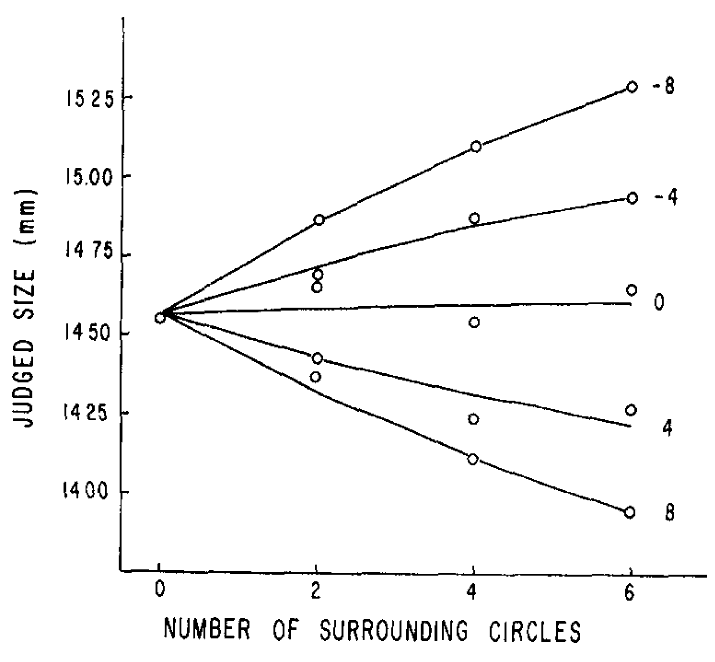
\includegraphics[width=0.55\textwidth]{Figures/Ebb_Variables} 
\decoRule
%\caption[Efecto del Numero y Tamaño de los círculos externos sobre la intensidad de la Ilusión de Ebbinghaus]{Se muestra el efecto que tienen el número de círculos externos incluídos en la ilusión de Ebbinghaus (eje x) sobre los fallos en la estimación del tamaño del círculo central (eje Y); se muestran con líneas diferentes los resultados obtenidos por ilusiones de Ebbinghaus donde los círculos externos diferían en tamaño del círculo central con los valores especificados. La figura fue extraída de la investigación conducida por \parencite{Massaro1971}; Figura 2}
\caption[Efecto del Número y Tamaño de los círculos externos en la intensidad de la Ilusión de Ebbinghaus]{Se presentan los resultados obtenidos en un experimento donde se manipuló el número y tamaño de los círculos externos de figuras de Ebbinghaus para evaluar su efecto sobre la intensidad de la ilusión perceptual evocada. La gráfica muestra el estimado del diámetro del círculo central de las figuras presentadas (promediando los datos obtenidos por todos los participantes y por los dos tamaños de círculo central usados: 13 y 17 mm), a través de los distintos niveles de número de círculos externos evaluados (eje de las abscisas) y por cada uno de los cinco tamaños de círculos externos utilizados (mostrados en líneas separadas). La tendencia de las líneas a alejarse del estimado promedio en ausencia de círculos externos -sin ilusión inducida- sugiere que a mayor número de círculos externos, mayor es la intensidad de la ilusión. La distancia vertical entre las líneas dibujadas parece indicar que la intensidad de la ilusión aumenta mientras mayor sea la diferencia entre el diámetro del círculo central y el de los círculos externos. \parencite{Massaro1971}.}
\label{fig:Ebb_Var}
\end{figure}

%Las condiciones de dificultad estarán determinadas por el número de círculos externos
Tomando en consideración los hallazgos reportados respecto de la influencia que tienen las variables inmersas en las figuras de Ebbinghaus sobre la ilusión perceptual asociada a las mismas \parencite{Massaro1971}, se decidió construir las dos condiciones de discriminabilidad para nuestra tarea de detección perceptual en búsqueda del Efecto Espejo, manipulando el número de círculos externos. Es decir, para que en la tarea de detección propuesta existiera una condición fácil -con una d' grande- se construyeron figuras de Ebbinghaus con 'pocos' círculos externos (2 o 3 círculos); y para la condición difícil -con una d' menor- se diseñaron figuras con 'muchos' círculos externos (7 u 8 círculos).\\ 

\subsection{Diseño de los Estímulos}

%En el experimento se trabajó con figuras de Ebbinghaus que promovieran efecto de subestimación Y sobrestimación del tamaño. 
En el diseño de las figuras de Ebbinghaus a utilizar en los experimentos propuestos se incluyeron los efectos de sobrestimación y de subestimación. Para ello se manejaron sólo dos tamaños de círculos externos, elegidos arbitrariamente de manera que fueran o más grandes que todos los tamaños de círculo central o más pequeños que la mayoría (5 cm y 1 cm).\\

%No se controló la distancia entre el círculo central y los círculos externos.
En ningún experimento se controló la distancia entre los círculos centrales y el halo de círculos externos. Los círculos externos fueron acomodados de acuerdo a los números de círculos externos considerados como parte de la condición difícil (siete y ocho), distribuyéndolos de manera uniforme y equidistante en torno al círculo central. Estos halos de siete y ocho círculos externos fueron usados como base para la construcción de los estímulos de la condición fácil (con dos o tres círculos externos), eliminando círculos y respetando la ubicación de los restantes. Este procedimiento se realizó para las figuras con efecto de subestimación y sobrestimación. Se procuró que en las figuras con dos círculos externos, estos estuvieran enfrentados en puntos opuestos del círculo central y en las figuras con tres círculos centrales, que rodearan al círculo central en ángulos de ciento veinte grados. La configuración de los halos de círculos externos resultantes permaneció constante para todos los tamaños de círculo central, haciendo que la distancia entre ambos elementos sea distinto para cada valor.\\

%El diámetro de los círculos centrales de las figuras de Ebbinghaus podía ser de 1 a 3 cm, en saltos de 0.5 cm
En ambos experimentos se utilizaron cinco valores para el tamaño de los círculos centrales (de 1 a 3 cm, en saltos de 0.5 cm). Cabe señalar que el diámetro elegido para los círculos externos en las ilusiones de sobrestimación (1 cm) es el mismo que el círculo central más pequeño. Sin embargo, esto no se considera un problema para la presente investigación porque la inclusión de los dos efectos (sobrestimación y subestimación) se hizo con la intención de prevenir la habituación y la fatiga de los participantes a la tarea, proveyendo a la misma de cierto dinamismo. El objetivo principal de la investigación realizada fue comparar el desempeño de los participantes entre las condiciones de discriminabilidad construidas con base en la literatura, y este tipo de figuras 'anómalas' se presentan de igual manera en ambas condiciones.\\

A continuación, se desarrolla con detalle la construcción de los estímulos y la distinción entre los tipos de ensayo (señal y ruido) aplicadas en cada uno de los dos experimentos llevados a cabo. Las especificaciones respecto al procedimiento y los controles realizados se explican con detalle más adelante.\\

\begin{itemize}
\item Experimento 1 : Circulo de referencia aislado vs Figura de Ebbinghaus.

%Los ensayos de la tarea de detección están compuestos por un círculo aislado constante del lado izquierdo, cuyo tamaño debe ser comparado con el círculo central de una figura de Ebbinghaus en el lado derecho de la pantalla.
En el Experimento 1 se mostró en cada ensayo una figura de Ebbinghaus en la mitad derecha de la pantalla, cuyo círculo central debía ser comparado por los participantes con un círculo de referencia aislado y con un diámetro constante de 2 cm localizado en el lado izquierdo de la pantalla. La tarea de los participantes consistía en presionar la tecla 'S' cuando ambos círculos fueran del mismo tamaño (señal) y la tecla 'N'  cundo no (ruido). Los círculos se mostraban a la misma altura de la pantalla, 14 cm a la izquierda y 10 cm a la derecha del centro de la pantalla.\\

%Desarrollo del diseño factorial de 5x2x2 utilizado para construir los estímulos del Experimento 1: 5 circulos centrales x 2 tipos de ilusion x 2 niveles de 'numero de circulos externos'
Las figuras de Ebbinghaus utilizadas en el Experimento 1 se diseñaron de acuerdo a un diseño factorial de 5x2x2, (Ver Figura~\ref{fig:Exp_1}). Se utilizaron cinco tamaños de círculo central que, partiendo del tamaño del círculo de referencia (2 cm; la combinación con la señal), se alejaban del mismo en saltos de 0.5 cm en ambas direcciones (i.e. Círculos más pequeños que la referencia, de 1 y 1.5 cm, y círculos más grandes que la referencia, de 2.5 y 3 cm de diámetro). Por cada uno de estos cinco tamaños de círculo central, se construyeron dos tipos de figuras de Ebbinghaus dependientes del tamaño de los círculos externos: grande (5 cm; efecto de subestimación) y pequeño (1 cm; efecto de sobrestimación). Y por último, por cada una de estas 10 combinaciones, se hicieron cuatro figuras diferentes de acuerdo a los niveles de 'número de círculos externos' propuestos por condición (2 y 3 círculos en la condición fácil; 7 y 8 círculos en la condición difícil). Esto nos deja con un subtotal de 20 figuras diferentes por condición y un total de 40 en todo el experimento.\\
 
%Los estímulos con ruido se presentaron 10 veces durante el experimento. Los estímulos con señal se presentaron con 40 repeticiones. La discrepancia en el número de repeticiones entre ambos tipos de estímulo se hizo para igualar la muesta de ensayos con señal y ensayos con ruido.
El conjunto de figuras de Ebbinghaus resultante contiene una mayor cantidad de estímulos con ruido (32 figuras con ruido; 16 por condición) que con señal (8 figuras con la señal; 4 por condición). Para igualar la cantidad de ensayos con señal y con ruido presentados a los participantes y preveer que la diferencia en su tasa de aparición pudiera sesgar su desempeño hacia la emisión de respuestas negativas, las figuras con señal diseñadas se repitieron un mayor número de veces que las figuras con ruido. Cada una de las 32 figuras de Ebbinghaus con ruido se presentó con diez repeticiones durante el experimento, mientras que las ocho figuras con señal tuvieron cuatro veces más repeticiones (40 en total). De esta forma, el experimento terminó compuesto por 320 ensayos con ruido y 320 ensayos con señal, 160 por cada condición de dificultad.\\

%Las repeticiones de cada figura aparecieron en cinco colores diferentes para prever la fatiga.
Los 640 estímulos contemplados en el Experimento 1 fueron presentados de manera aleatoria. Procurando evitar la fatiga de los participantes, las repeticiones de los estímulos diseñados se mostraron en cinco colores diferentes (Guinda, Anaranjado, Verde, Azul y Púrpura) en cantidades iguales (dos repeticiones de cada color para los estímulos con ruido y ocho para los estímulos con señal).\\

\item Experimento 2 : Figura de Ebbinghaus vs Figura de Ebbinghaus.

%En la tarea de detección, los participantes tenían que comparar el círculo central de dos figuras de Ebbinghaus que aparecían simultáneamente en la pantalla: una con círculos externos grandes (Efecto de subestimación)  y una con círculos externos pequeños (Efecto de sobrestimación).
En el Experimento 2 los participantes tenían que comparar el diámetro del círculo central de dos figuras de Ebbinghaus mostradas simultáneamente en pantalla y, al igual que en el Experimento 1, presionar la tecla 'S' cuando fueran del mismo tamaño (señal) y la tecla 'N' cuando no (ruido). Las parejas construidas estaban compuestas por una figura de Ebbinghaus con efecto de subestimación (con círculos externos grandes, de 5 cm de diámetro) y una figura con efecto de sobrestimación (con círculos externos pequeños, de 1 cm de diámetro). Los círculos centrales aparecían en pantalla a la misma altura, 15 cm a la izquierda y 11 cm a la derecha del centro de la pantalla.\\


%Se formaron cinco parejas con la Señal (cinco pares iguales de tamaño de círculo central) y cinco parejas con el ruido (cuatro cuyos círculos centrales diferían en 0.5 cm y una que difería en 1 cm).
La Figura~\ref{fig:Exp_2} ilustra el diseño de las figuras de Ebbinghaus utilizadas en el Experimento 2. A diferencia del Experimento 1, donde uno de los círculos a comparar era constante, en el Experimento 2 se varió el diámetro de los dos círculos a comparar. Para ello se ello se utilizaron los mismos cinco tamaños de círculo central (de 1 a 3 cm en saltos de 0.5 cm) y por lo tanto, con cinco combinaciones posibles para las Parejas-señal. Así mismo, se formaron cinco Parejas-ruido juntando arbitrariamente valores de círculo central que guardasen una diferencia de 0.5 cm entre sí -1 vs 1.5; 1.5 vs 2; 2 vs 2.5 y 2.5 vs 3 cm- con una quinta pareja con una diferencia de 1 cm entre los valores de círculo central intermedios -1.5 cm vs 2.5 cm-. Por cada una de estas 10 parejas, se crearon cuatro variaciones por condición, de acuerdo con las combinaciones posibles de niveles de 'número de círculos externos' (2 círculos externos a ambos lados, 3 círculos externos a ambos lados, 2 en izquierdo y 3 en derecho, y 3 en izquierdo y 2 en derecho en la condición fácil; 7 círculos externos a ambos lados, 8 círculos externos ambos lados, 7 círculos del lado izquierdo y 8 en el derecho y 8 círculos en el lado izquierdo y 7 en el derecho en la condición difícil). En total, el Experimento 2 estuvo compuesto por 80 parejas diferentes de figuras de Ebbinghaus cuyos círculos centrales debían compararse, 40 con la señal y 40 con el ruido y 20 de cada uno por condición.\\

%Cada pareja diseñada se repitió 8 veces; en 4 colores diferentes y contrabalanceando la ubicación de cada tipo de ilusión. En total, el Experimento 2 estuvo compuesto por 640 ensayos.
Cada una de las 80 parejas diseñadas para el Experimento 2 se presentó 8 veces, en cuatro colores diferentes (púrpura, anaranjado, azul y verde) para prevenir la fatiga de los participantes y contrabalanceando la ubicación de las ilusiones de sobrestimación y subestimación a la derecha o izquierda de la pantalla. Es decir, por cada pareja construida de figuras a comparar se incluyeron ocho ensayos en el experimento: un par de cada uno de los cuatro colores propuestos y dentro de estos, se contrabalanceó la localización de las figuras con efecto de sobrestimación y subestimación. De tal forma que el Experimento 2 estuvo compuesto por un total de 640 ensayos, 320 por cada tipo de ensayo (ruido y señal) y 160 por cada condición.\\ 

\subsection{Materiales}

%Programacion de la tarea
La tarea fue programada y ejecutada en PsychoPy v.12, un paquete de libre acceso diseñado para facilitar la generación de tareas experimentales en psicología y neurociencias con el lenguaje de programación Python.\\

%Detalles sobre la Mac y el espacio utilizado para correr el experimento.
El experimento se corrió en una computadora de escritorio Mac (pantalla de 59.5 x 34 cm), en un cubículo dentro del laboratorio 25 del Edificio D de la Facultad de Psicología de la UNAM. \\

%Los participantes se sentaron a 1.10 m de distancia de la pantalla
Los participantes se sentaron en una silla fija, situada a 1.10 m de distancia de la pantalla.\\ 


\subsection{Participantes}

%Total de participantes y distribucion entre experimentos.
Un total de cuarenta y un estudiantes de la Facultad de Psicología participaron en uno de los experimentos: veinte en el Experimento 1 y veintiuno en el Experimento 2. Los experimentos se llevaron a cabo de manera simultánea, asignando a los participantes alternadamente a uno de ellos, procurando terminar con una cantidad similar de participantes en cada uno. Los participantes nunca tuvieron conocimiento de que existiera más de un experimento.\\

%Procedencia y generalidades sobre los participantes.
Los participantes eran estudiantes de los primeros cuatro semestres de la licenciatura en Psicología en la Facultad de Psicología de la Universidad Nacional Autónoma de México, con edades entre los 18 y los 21 años. Se incentivó su participación ofreciéndoles a cambio un boleto para la rifa de una tarjeta de regalo con valor de \$300 pesos para utilizarse en la plataforma de su preferencia entre iTunes, Netflix y Amazon. Los participantes tenían visión normal o corregida hacia lo normal.\\ 

%Consentimiento informado.
Previo a su participación en el experimento se solicitó a los participantes que firmaran una carta de consentimiento donde se les informó la duración estimada de la tarea (40 minutos para cualquiera de los experimentos), se reiteraba su participación en una rifa y se les advertía de la fatiga que podrían experimentar durante el procedimiento y que, aunque su participación era voluntaria y podían dimitir en cualquier momento, se les solicitaba encarecidamente que permanecieran hasta el final dado que de lo contrario no se podrían utilizar sus datos.\\

\section{Procedimiento}

%Los experimentos propuestos difieren en el tipo de estímulos a presentar. Sin embargo, la tarea principal y el resto de los detalles del procedimiento permanecen iguales para ambos casos. 
La única diferencia entre los Experimentos 1 y 2 fue el tipo de estímulos presentados a los participantes para su comparación: en un caso se enfrentó el círculo central de una figura de Ebbinghaus contra un círculo de referencia fijo (Experimento 1) y en el otro, se mostraron simultáneamente dos figuras de Ebbinghaus (Experimento 2). Sin embargo, en ambos casos la tarea de detección perceptual es la misma (comparar el diámetro de dos círculos específicamente señalados en la pantalla para determinar si éstos eran -o no- del mismo tamaño), así como el procedimiento y su programación.\\

%La tarea de detección constaba de dos fases: 1) Una tarea de detección binaria (¿Son o no del mismo tamaño?) y 2) Una tarea con escala de confianza (¿Qué tan seguro estás de tu respuesta?)
La tarea de detección planteada se evaluó mediante dos procedimientos diferentes: 1) una pregunta binaria 'Sí/No' y 2) la puntuación de esta respuesta en una escala de confianza con valores del 1 al 3 ('1' siendo 'poco seguro' y '3', 'muy seguro'), que de acuerdo a su correspondencia con la respuesta dada em la fase binaria se transformaría y registraría en términos de una escala más informativa, con valores del 0 al 6, ('0' siendo 'totalmente seguro que no eran iguales' y '6', 'totalmente seguro que sí lo eran').\\

Tras firmar la carta de consentimiento informado, se instaló a cada participante en el espacio asignado para la realización del experimento, donde el monitor mostraba una pantalla de bienvenida que incluía la leyenda "Presiona la barra espaciadora para comenzar con las instrucciones". En el Apendice $WAWAWAWA$ se presentan capturas de pantalla que presentan las instrucciones dadas a los participantes tal y como aparecieron en el experimento. Las instrucciones finalizaban con una pantalla en blanco donde se leía 'Presiona la barra espaciadora para comenzar el experimento', dando a los participantes control sobre el momento en que se sintieran listos para comenzar el experimento.\\

El experimento se extendia a lo largo de 640 ensayos, (uno por cada estímulo construido). A continuación, se detalla la estructura de cada uno de los ensayos:\\

\begin{itemize}
\item Fase 1: Tarea de respuesta binaria 'Sí/No'

Cada ensayo comenzaba con la presentación de los estímulos a comparar, acompañados por un par de leyendas que recordaban a los participantes la pregunta de detección a responder -"¿Los círculos centrales son del mismo tamaño?"- y las teclas que debían presionar para emitir su respuesta -"S = Sí, N = No"-, en la parte superior e inferior de la pantalla, respectivamente. La Figura~\ref{fig:Ejem_YN} presenta un ejemplo de cómo se presentaban los estímulos a comparar durante la fase de respuestas binarias, por cada condición y por cada efecto-ilusión incluído en el Experimento 1.\\

\begin{figure}[th]
\centering
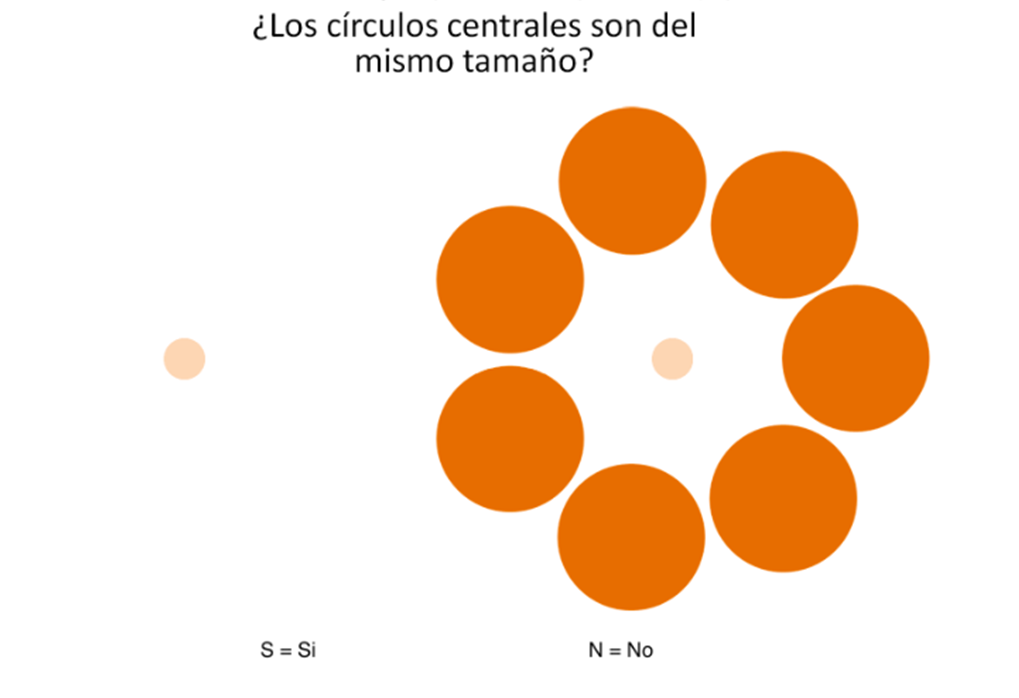
\includegraphics[width=0.5\textwidth]{Figures/Ejemplo_EnsayoYN_1} 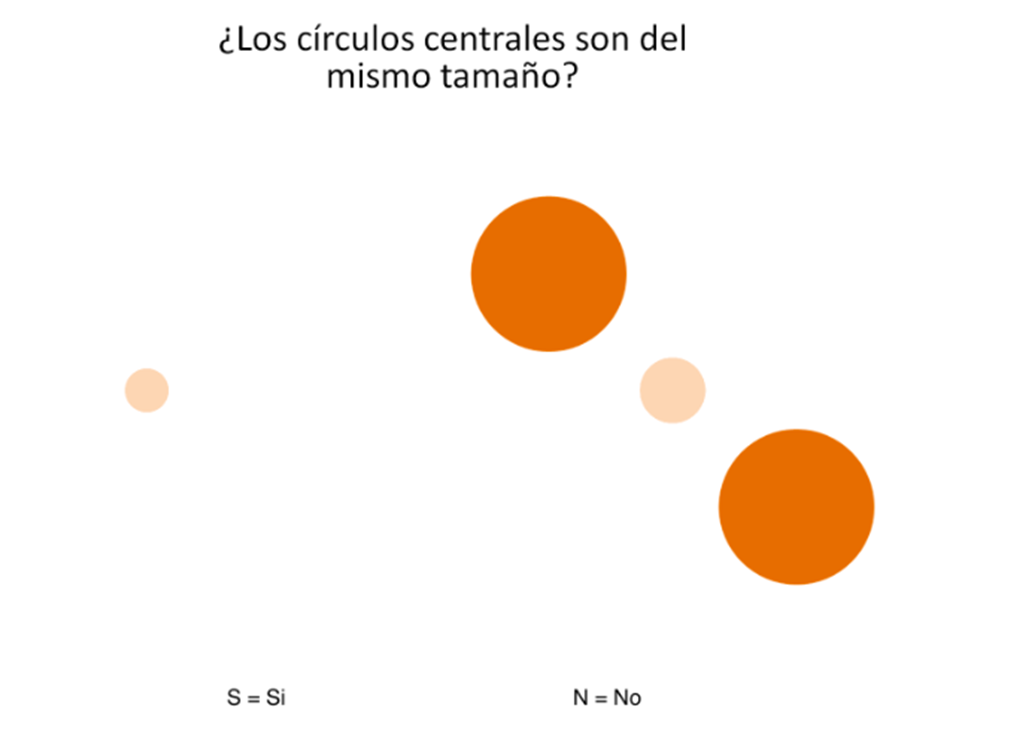
\includegraphics[width=0.5\textwidth]{Figures/Ejemplo_EnsayoYN_2}
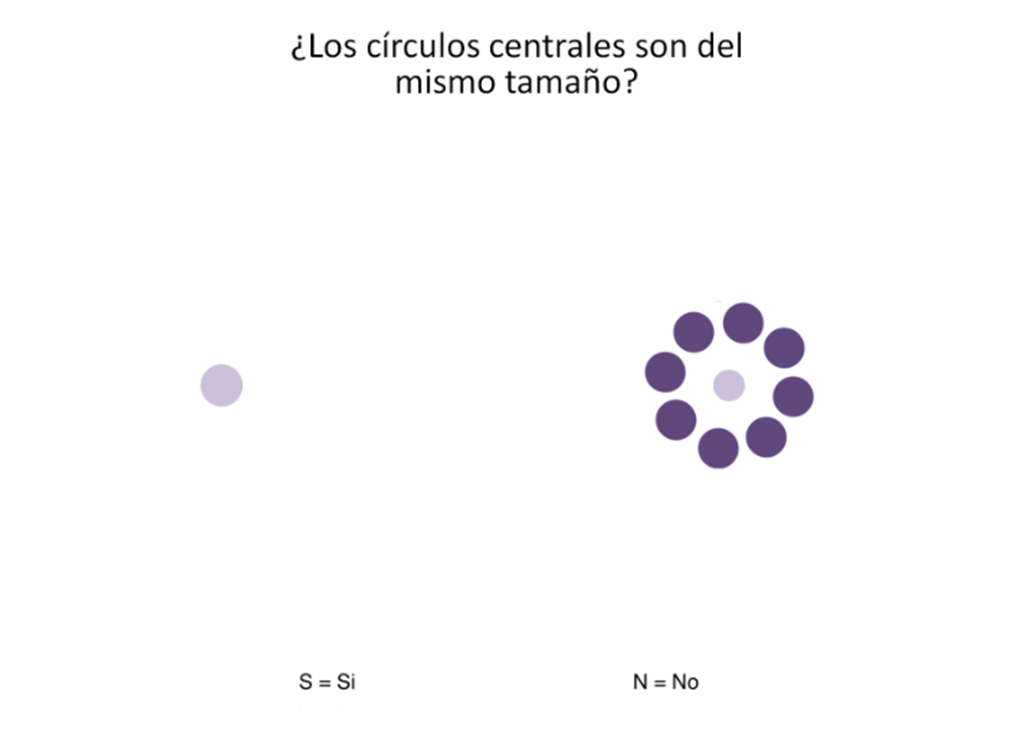
\includegraphics[width=0.5\textwidth]{Figures/Ejemplo_EnsayoYN_4} 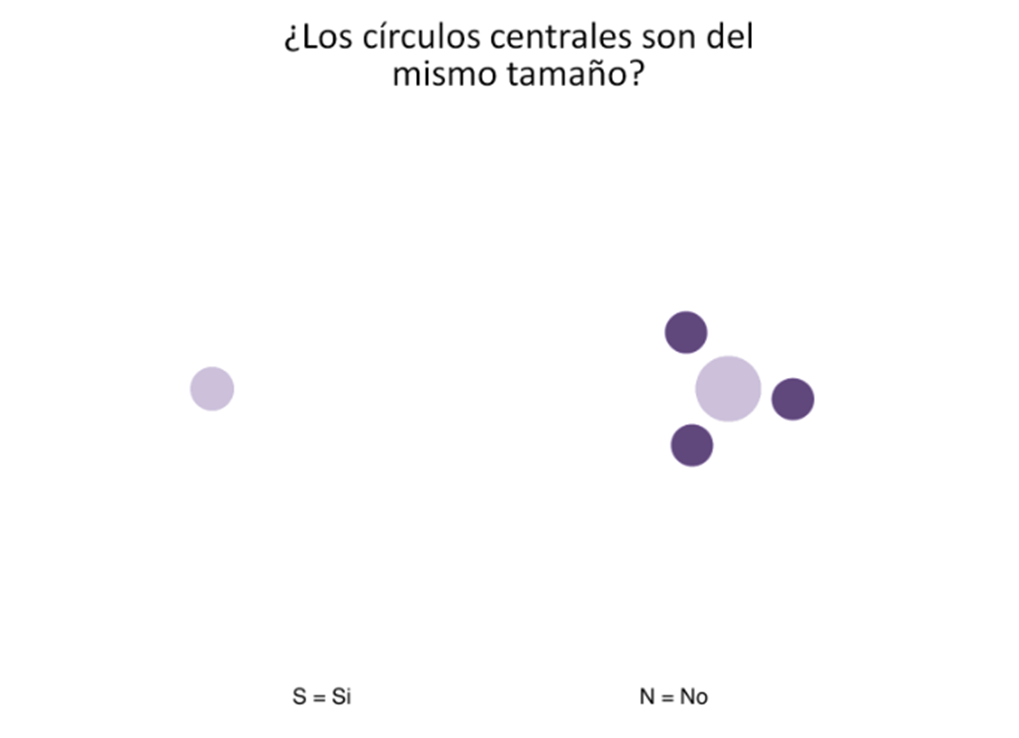
\includegraphics[width=0.5\textwidth]{Figures/Ejemplo_EnsayoYN_3}
%\decoRule
\caption[Presentación de ensayos con tarea de detección binaria]{Se muestran cuatro ejemplos de la tarea de detección binaria, tal y como se les presentó a los participantes. Los paneles izquierdos presentan estímulos pertenecientes a la condición difícil y los paneles derechos, a la condición fácil. Los paneles superiores muestran ilusiones con efecto de subestimación y los paneles inferiores, con efecto de sobrestimación.}
\label{fig:Ejem_YN}
\end{figure}

Los estímulos permanecían en pantalla durante 1.5 segundos con independencia de si los participantes habían, o no, emitido una respuesta: Si el participante respondía antes, los estímulos se quedaban en pantalla hasta cumplirse el intervalo, tras el cual se pasaba inmediatamente a la segunda fase del ensayo; si el participante no había respondido, los recordatorios permanecían solos en pantalla hasta que se registrara una respuesta. Esta restricción fue incluida para preveer la posibilidad de que los participantes se habituaran a la ilusión al prolongar su observación.\\

\item Fase 2: Escala de Confianza

%En una segunda fase, los participantes tuvieron que oprimir una tecla del 1 al 3 para indicar qué tan seguros estaban de la respuesta recién emitida.
Una vez registrada la respuesta de los participantes a la tarea 'Sí/No', se les mostró una segunda pantalla donde se les solicitaba que indicaran qué tan seguros se sentían de la respuesta binaria recién dada, de acuerdo con la escala presentada en pantalla, oprimiendo la tecla '1', '2' ó '3', (ver Figura~\ref{fig:Ejem_Esc}). \\

Los puntajes registrados por los paricipantes -'1','2' o '3'- se tradujeron y registraron en una escala más grande -con valores del 1 al 6- que separa en direcciones opuestas la confianza que se tiene en los juicios de detección posibles, es decir, distingue entre la confianza que se tiene en que el estímulo evaluado contenga sólo ruido ('1 = Muy seguro de que NO son iguales'; '2 =  Más o menos seguro de que NO son iguales'; '3 = Poco seguro de que NO son iguales') y la confianza de que se trate de un estímulo con señal ('4 = Poco seguro de que son iguales'; '5 = Más o menos seguro de que son iguales'; '6 = Muy seguro de que son iguales'). La conversión de los puntajes emitidos a la escala de seis elementos se realizó en función a la respuesta binaria recién registrada, de la siguiente forma:

\begin{itemize}
\item En los ensayos en que el participante hubiera respondido 'No' a la pregunta de detección binaria '¿Los círculos centrales son del mismo tamaño?', la conversión de los puntajes de confianza asignados sería:\\
	\begin{itemize}
	\item '3 = Estoy muy seguro de mi respuesta', se traduciría en '1'.\\
	\item '2 = Estoy más o menos seguro de mi respuesta', habría conservado el valor '2'.\\
	\item '1 = Estoy poco seguro de mi respuesta', se convertiría en '3'.\\
	\end{itemize}
\\
\item En los ensayos donde el participante hubiera respondido 'Sí' en la primera fase, la transformación de los puntajes asignados habría sido la siguiente:\\
	\begin{itemize}
	\item '1 = Estoy poco seguro de mi respuesta', se transformaría en '4'.\\
	\item '2 = Estoy más o menos seguro de mi respuesta', se registraría como '5'.\\
	\item '3 = Estoy muy seguro de mi respuesta', se convertiría en '6'.\\
	\end{itemize}
\end{itemize}\\

De tal forma que los valores extremos de la escala construida representan una mayor seguridad en las respuestas emitidas en la fase anterior -'Sí' o 'No'- y los valores intermedios, una mayor incertidumbre.\\

\begin{figure}[th]
\centering
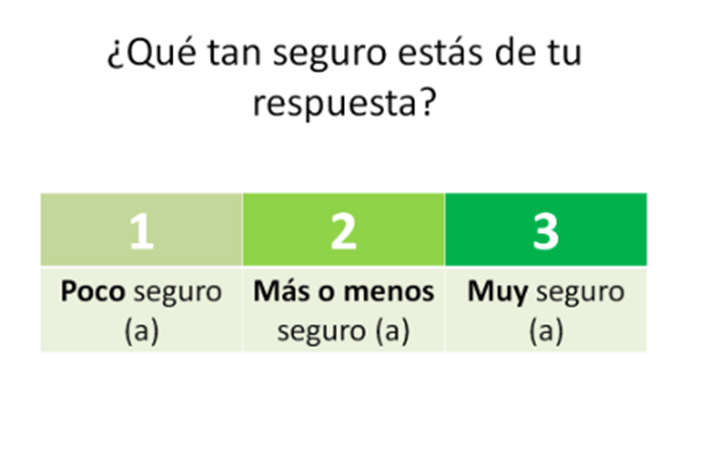
\includegraphics[width=0.55\textwidth]{Figures/Ejemplo_Escala}
%\decoRule
\caption[Presentación de la escala de confianza]{La escala de confianza mostrada a los participantes en la segunda fase de la tarea y  a partir de la cual se les solicitaba evaluar e indicar qué tan seguros se sentían del juicio de detección emitido con su respuesta inmediatamente anterior}
\label{fig:Ejem_Esc}
\end{figure}\\

Una vez registrada la segunda respuesta del participante -el puntaje asignado en la escala de confianza- se daba por terminado el ensayo.\\

\end{itemize}

%Entre cada ensayo, se presentó una pantalla intermedia que solicitaba a los participantes presionar la barra espaciadora para indicar que estaban listos para responder al siguiente ensayo.
Entre ensayo y ensayo, se incluyó una pantalla 'de descanso' que indicaba a los participanes que debían presionar la barra espaciadora para continuar. Estas pantallas 'en pausa' otorgaban control a los participantes de su avance en el experimento y fueron incluídas para garantizar que estuvieran prestando atención durante la presentación -restringida en el tiempo- de los estímulos a comparar.\\

Al terminar los 640 ensayos, se mostraba una última pantalla donde se presentaba la retroalimentación general del desempeño de cada participante (Total de aciertos y errores cometidos), únicamente con el fin de dar cierto sentido de 'conclusión' a su participación. En ningún momento se informó a los participantes sobre el propósito de la investigación, ni sobre la existencia de los niveles de dificultad entre los cuales se compararía su ejecución.\\ 

%Se registraron tiempos de respuesta por cada respuesta registrada (Respuesta en la tarea Sí/No; Respuesta en la escala de confianza) y  la duración del experimento completo.
Además de las respuestas dadas por los participantes, se registraron también los tiempos de respuesta a lo largo del experimento (latencias). En el Apéndice $APENDICE$ se muestra y desarrolla en detalle cuáles fueron los datos obtenidos y registrados por cada uno de los participantes.\\

\begin{figure}[th]
\centering
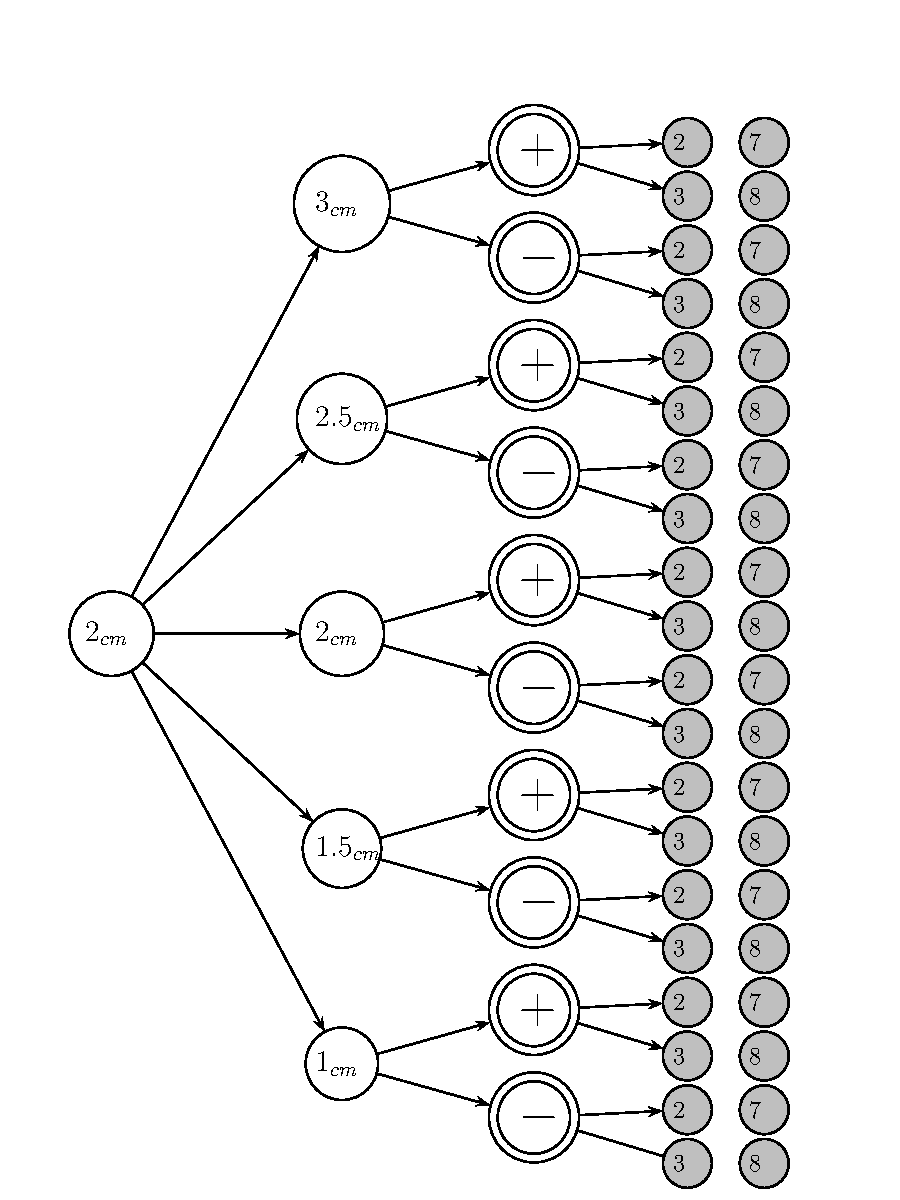
\includegraphics[width=0.99\textwidth]{Figures/Estimulos_Experimento1} 
\decoRule
\caption[Diseño de Estimulos en el Experimento 1]{Ilustración del diseño factorial 5x2x2 utilizado para construir las figuras de Ebbinghaus presentadas en el Experimento 1. En cada ensayo los participantes compararon el tamaño de un círculo de referencia constante (2cm de diámetro, ilustrado en el lado izquierdo de la figura) con el círculo central de una figura de Ebbinghaus que podía ser de cinco tamaños diferentes, con círculos externos que inducieran efectos de sobrestimación o subestimación (señalados con signos positivos y negativos, respectivamente) y con dos variaciones del 'número de círculos externo' dependientes de la condición (2 y 3 círculos externos en la condición fácil o 7 y 8 en la condición difícil). Por cada condición, se tienen 16 estímulos con ruido, (repetidos 10 veces cada uno en cinco colores diferentes) y cuatro que contienen la señal (presentados 40 veces cada uno, en cinco colores diferentes), dejándonos con 320 ensayos por condición y un total de 640 ensayos en todo el experimento.}
\label{fig:Exp_1}
\end{figure}

\begin{figure}[th]
\centering
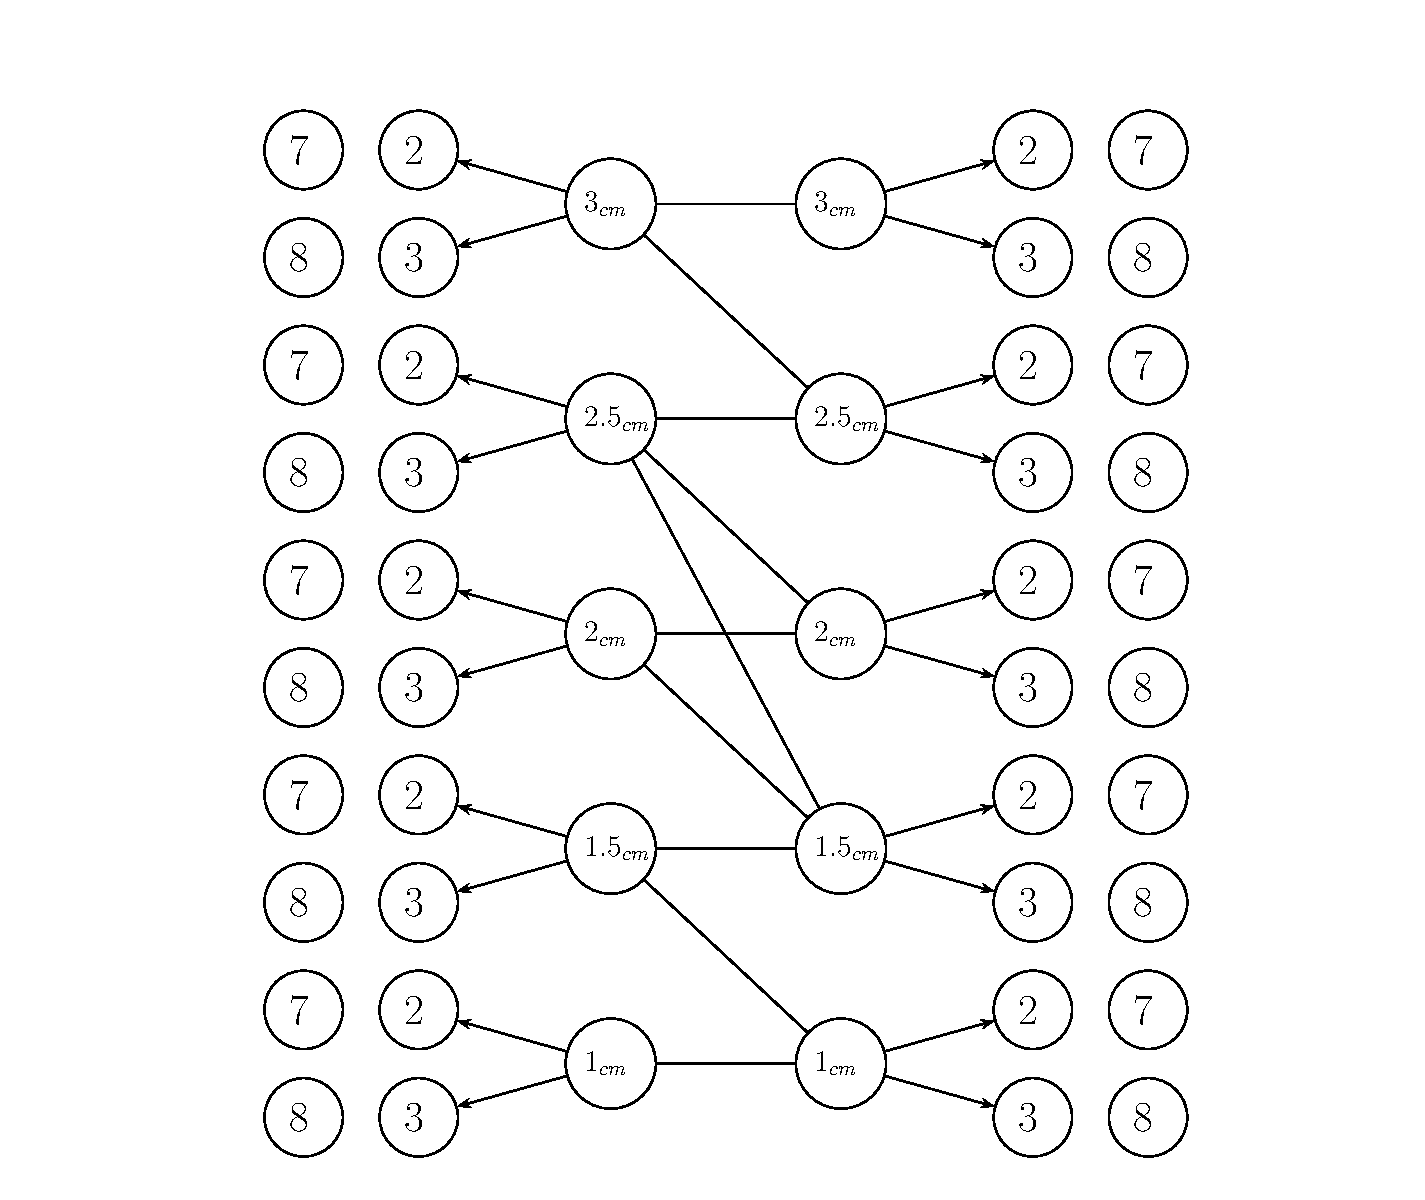
\includegraphics[width=0.9\textwidth]{Figures/Estimulos_Experimento2} 
\decoRule
\caption[Diseño de Estimulos en el Experimento 2]{Diseño de las parejas de figuras de Ebbinghaus mostradas en el Experimento 2, compuestas por una figura con efecto de subestimación y una con efecto de sobrestimación. Con los cinco tamaños distintos de círculo central propuestos se crearon cinco parejas iguales (señales) y cinco parejas arbitrarias desiguales (ruido). Por cada una de las diez parejas se consideró las cuatro combinaciones posibles entre los niveles de círculos externos incluídos en cada condición - 2 vs 2 o 7 vs 7; 3 vs 3 u 8 vs 8; 2 vs 3 o 7 vs 8; 3 vs 2 o 8 vs 7) Cada pareja se repitió ocho veces, contrabalanceando la posición derecha-izquierda de los efectos de sobrestimación y subestimación.}
\label{fig:Exp_2}
\end{figure}
\end{itemize}


